\documentclass{beamer}
\usepackage{latexsym} 
\usepackage{graphicx}
\usetheme{Warsaw}

\title{Chapter 4}
\subtitle{Data Preprocessing: Practical Issues}

\begin{document}
\maketitle

\begin{frame}
  \frametitle{Splitting data into train and test}
  \begin{itemize}
  \item Download wine dataset
    \begin{itemize}
    \item Three classes which map to different types of grapes in Italy
    \end{itemize}
  \item Cannot train and test on the same data
  \item So allocate some portion for testing and use the rest for training
    \begin{itemize}
    \item 70-30 or 80-20 split
    \end{itemize}
  \item Splitting three ways is a better idea to allocate some dev data
  \item N-fold cross-validation
  \item Scikit-learn helper methods (e.g. train\_test\_split())
  \item \href{https://github.com/rasbt/python-machine-learning-book/blob/master/code/ch04/ch04.ipynb}{Chapter 4 iPython notebook}
  \end{itemize}
\end{frame}

\begin{frame}
  \frametitle{Wine dataset}
  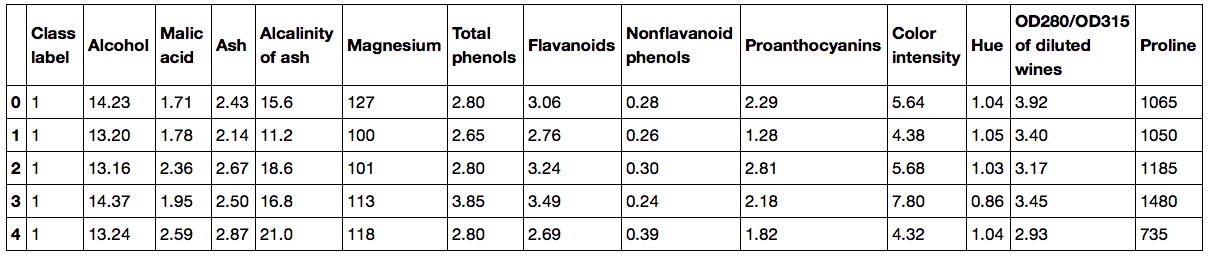
\includegraphics[width=\textwidth]{Code/ch04/images/04_10.png} 
\end{frame}

\begin{frame}
  \frametitle{Feature scaling}
  \begin{itemize}
  \item Imagine we have two features
    \begin{itemize}
    \item $1 < x_1 < 10$
    \item $1 < x_2 < 100000$
    \end{itemize}
  \item Algorithm will likely focus on optimizing $w_2$
  \item As this will produce the largest changes in perceptron error
  \item KNN based on Euclidean distance will be dominated by $x_2$
  \item Two common approaches
    \begin{itemize}
    \item Normalization
    \item Standartization
    \end{itemize}
  \end{itemize}
\end{frame}

\begin{frame}
  \frametitle{Normalization}
  \textit{Normalization} refers to the rescaling of the features to a range of [0, 1].  To normalize the data, we apply the min-max scaling to each feature column, where the new value $x_{norm}^{(i)}$ of a sample  $x^{(i)}$ is calculated as follows:
  \[
  x_{norm}^{(i)} = \frac{x^{(i)} - \mathbf{x}_{min}}{\mathbf{x}_{max} - \mathbf{x}_{min}}
  \]
  Here, $x^{(i)}$ is a particular sample, $x_{min}$ is the smallest value in a feature column, and $x_{max}$ the largest value, respectively.
\end{frame}

\begin{frame}
  \frametitle{Standartization}
  \begin{itemize}
  \item Normalization gives us values in a bounded interval
  \item Standartization can be more practical:
  \item Many ML algorithms initialize the weights to zero
  \item Standartization centers the columns at $mean=0$ and $std=1$
  \item So feature columns take the form of a normal distribution
  \item This makes it easer to learn the weights
  \item Standartization encodes useful info about outliers
  \item Vs. normalization which scales the data to a fixed range
  \end{itemize}
\end{frame}

\begin{frame}
  \frametitle{}
  The procedure of standardization can be expressed by the following equation:
  \[
  x_{std}^{(i)} = \frac{x^{(i)} - \mu_{x}}{\sigma_{x}}
  \]
  Here, $\mu_{x}$ is the sample mean of a particular feature column and $\sigma_{x}$ the corresponding standard deviation, respectively.
  \begin{itemize}
  \item \href{https://github.com/rasbt/python-machine-learning-book/blob/master/code/ch04/ch04.ipynb}{Example of using normalization and standardization}
  \end{itemize}
\end{frame}

\begin{frame}
  \frametitle{L1 regularization}
  Recall L2 regularization -- one approach to reduce model complexity
  \[
  L2: \lVert \mathbf{w} \rVert^{2}_{2} = \sum_{j=1}^{m} w^{2}_{j}
  \]
  An alternative approach is \textit{L1 regularization}:
  \[
  L1: \lVert \mathbf{w} \rVert_{1} = \sum_{j=1}^{m} |w_j|
  \]
\end{frame}

\begin{frame}
  \frametitle{L1 regularization}
  \begin{itemize}
  \item L1 yields sparse solutions
  \item Most feature weights will be zero
  \item Useful for high-dimensional datasets with irrelevant features
  \item It can be viewed as a technique for feature selection
  \item Some intuition as to why this is the case will follow
  \end{itemize}
\end{frame}

\begin{frame}
  \frametitle{L2 regularization}
  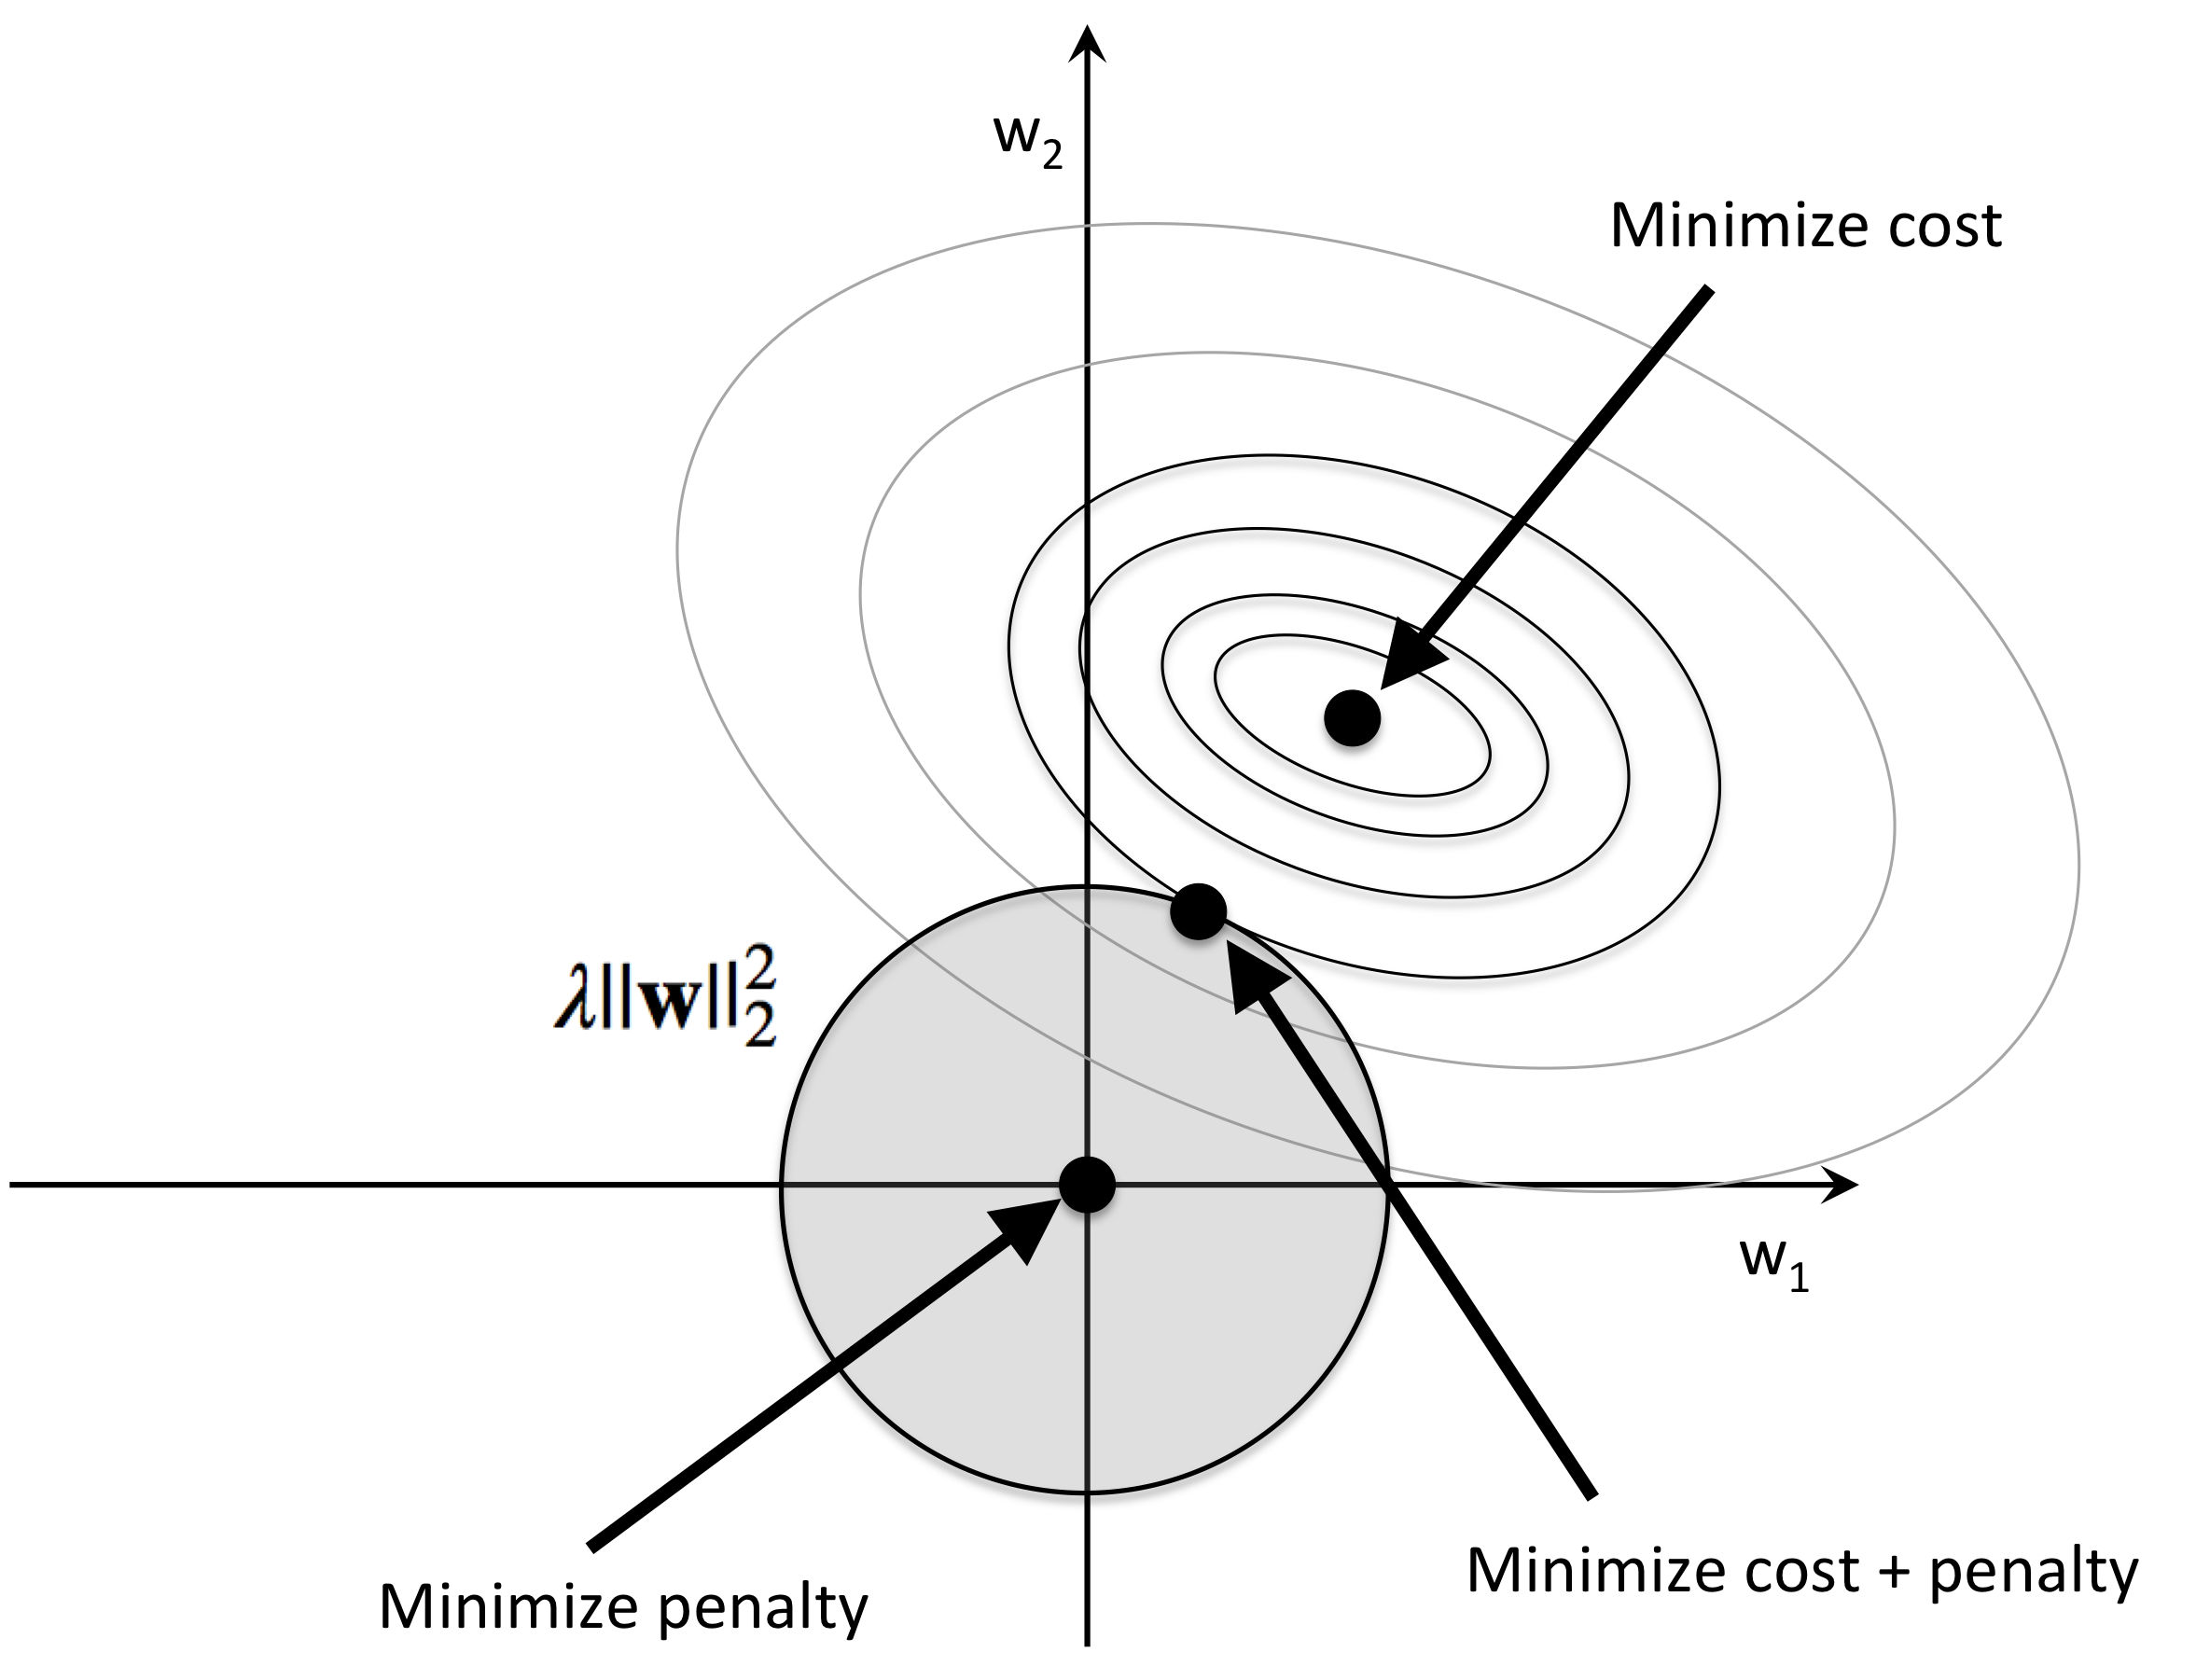
\includegraphics[width=\textwidth]{Code/ch04/images/04_12.png} 
\end{frame}

\begin{frame}
  \frametitle{L1 regularization}
  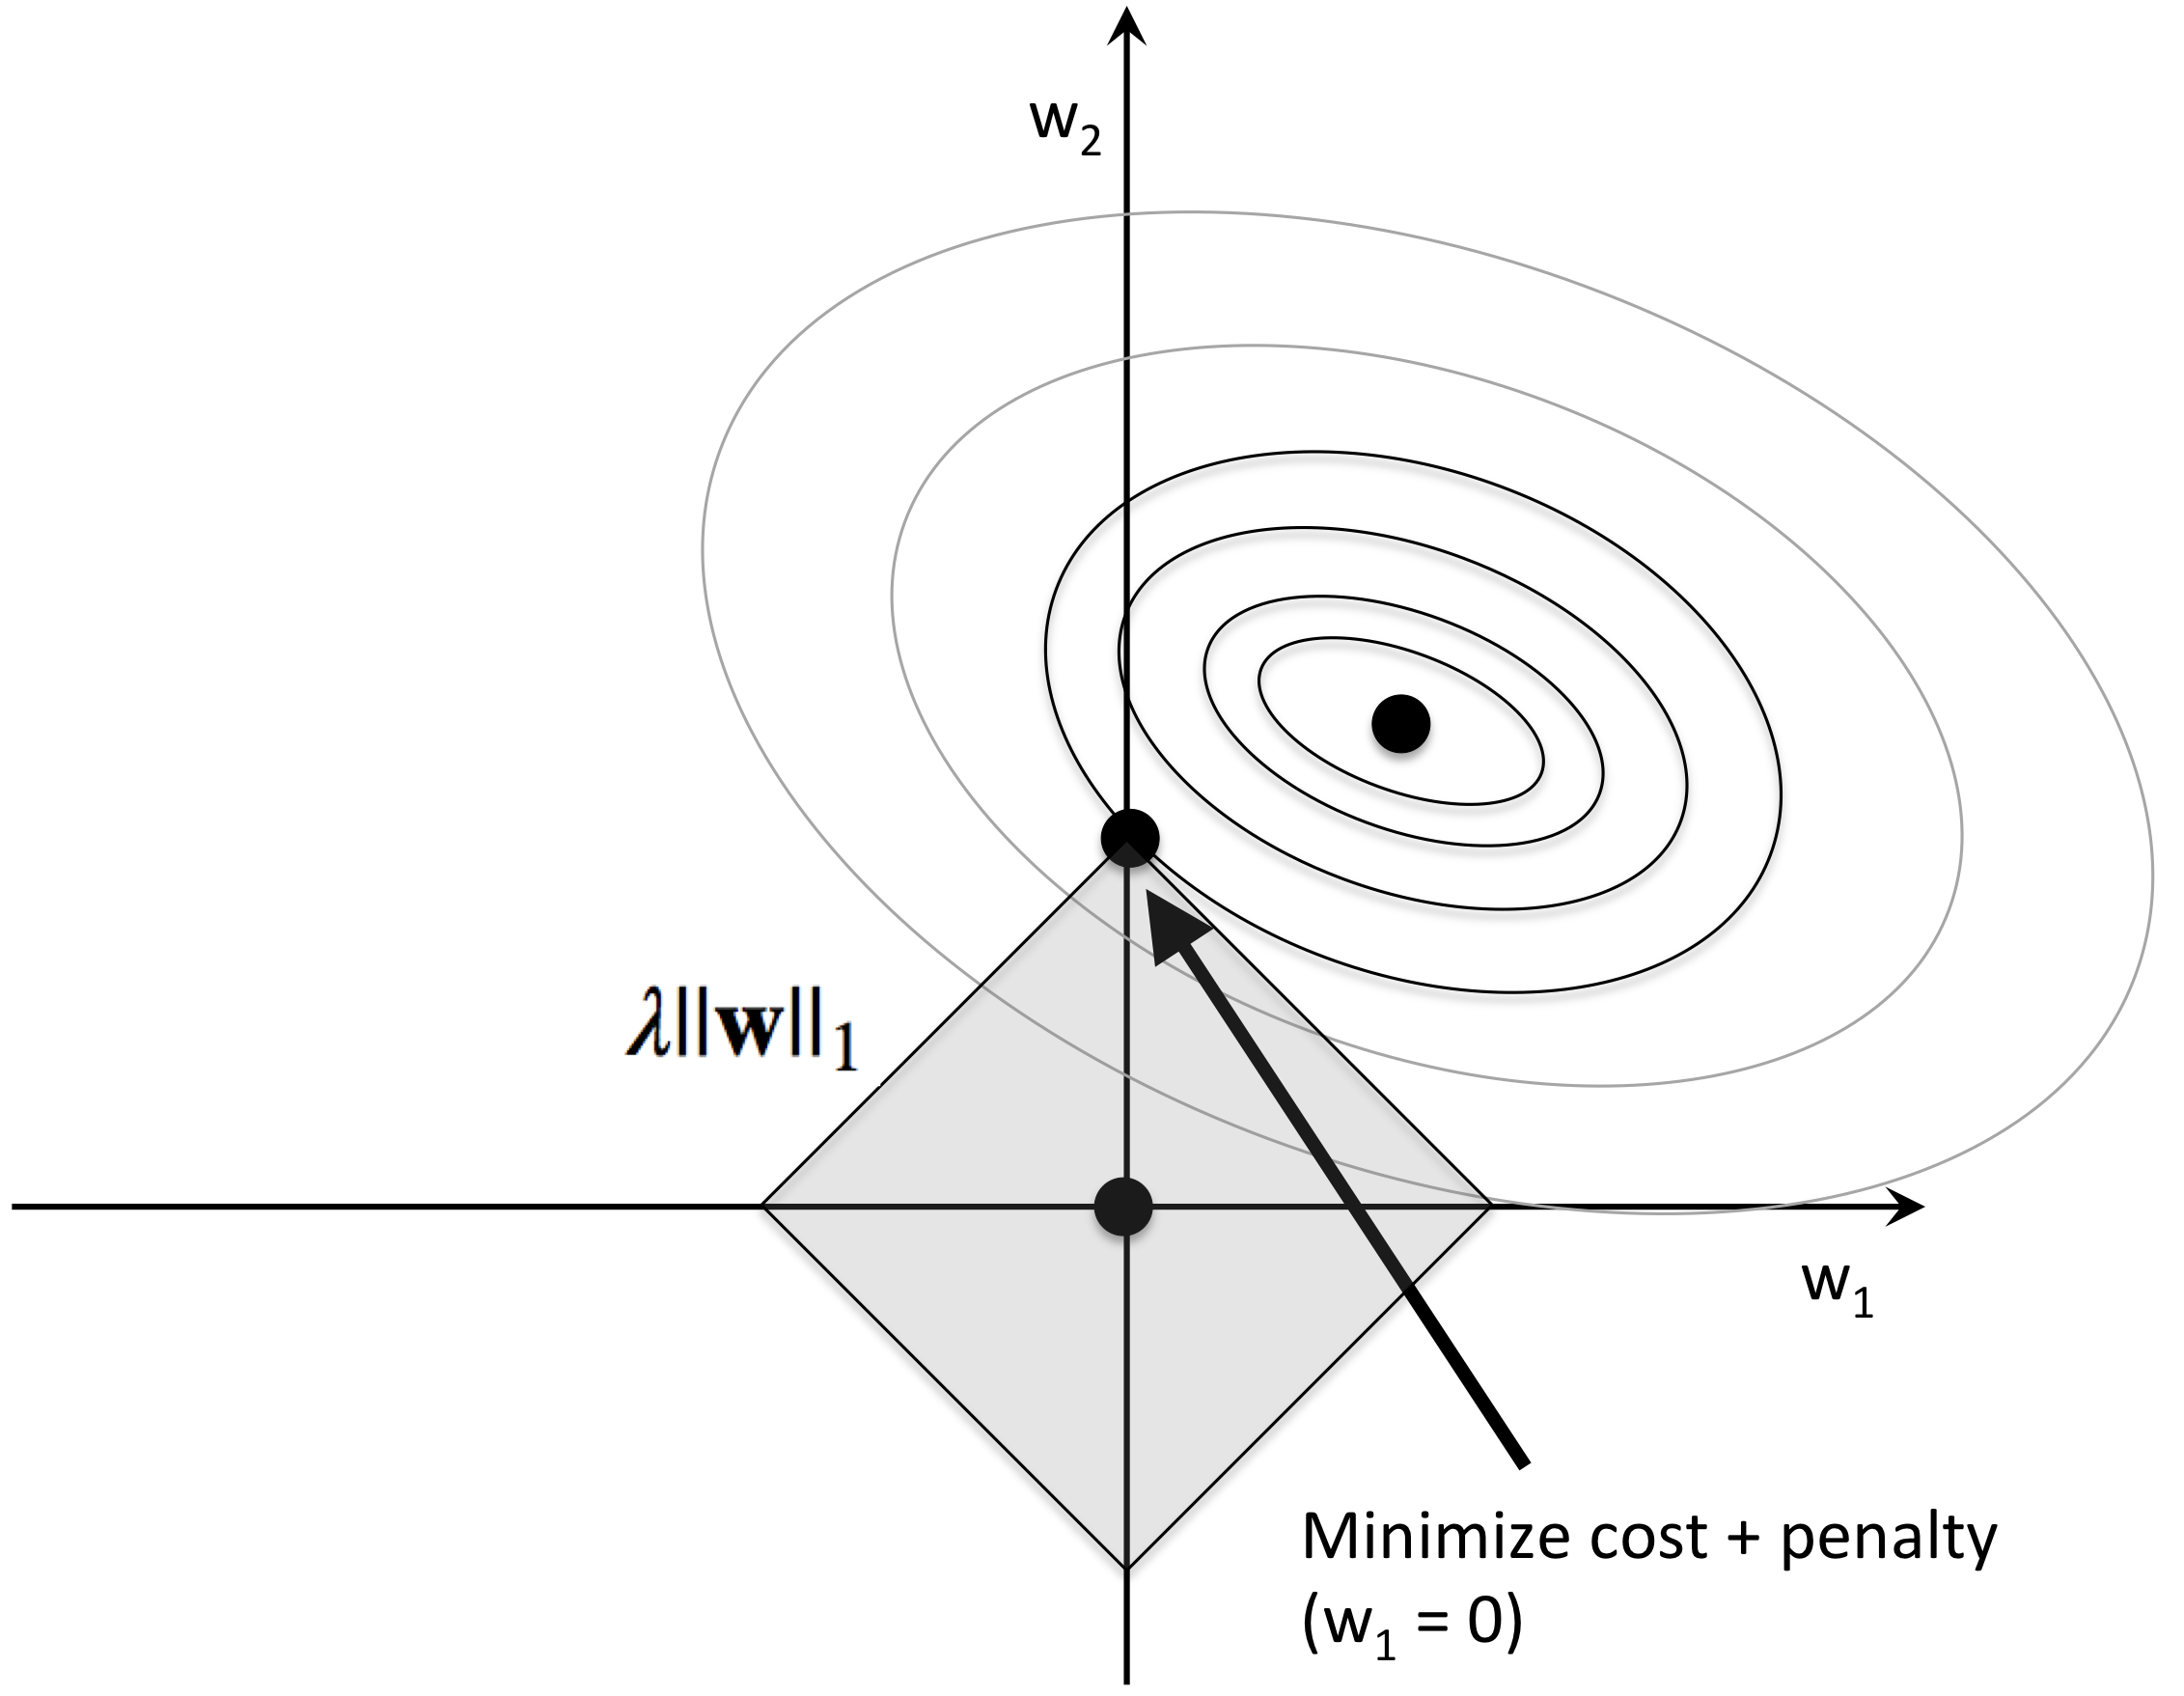
\includegraphics[width=\textwidth]{Code/ch04/images/04_13.png} 
\end{frame}

\begin{frame}
  \frametitle{Sparcity}
  \begin{itemize}
  \item Regularization penalty and cost pull in opposite directions
  \item Regularization wants the weight to be at (0, 0)
  \item I.e. regularization prefers a simpler model
  \item And decreases the dependence of the model on the training data
  \item \href{https://github.com/rasbt/python-machine-learning-book/tree/master/code/ch04}{L1 in scikit-learn}
  \end{itemize}
\end{frame}

\begin{frame}
  \frametitle{}
  \begin{itemize}
  \item 
  \end{itemize}
\end{frame}

\end{document}
